% Source: graduate-coursework/Prior_Semesters/Fa25/EMCH501/HW4/HW4.tex

\documentclass[border=4pt]{standalone}
\usepackage{amsmath}
\usepackage{amssymb}
\usepackage{graphicx}
\usepackage{pgfplots}
\usepackage{tikz}
\usepackage{xcolor}
\pgfplotsset{compat=1.18}
\usetikzlibrary{shapes.geometric, arrows.meta, positioning, decorations.pathmorphing, patterns}

\definecolor{USC_Garnet}{HTML}{73000A}
\definecolor{USC_Sandstorm}{HTML}{FFF2E3}
\definecolor{USC_Black90}{HTML}{565656}
\definecolor{USC_Black10}{HTML}{ECECEC}
\definecolor{USC_Honeycomb}{HTML}{65780B}
\definecolor{tablegreen}{RGB}{230,242,230}
\definecolor{outputbg}{RGB}{245,245,245}


\begin{document}
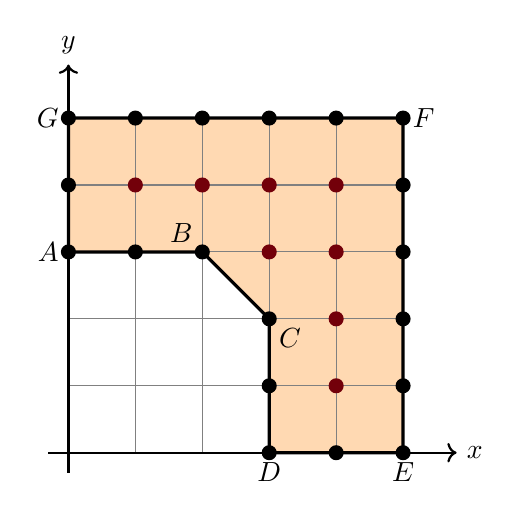
\begin{tikzpicture}[scale=0.85]
    % Fill the L-shaped region
    \fill[orange!30] (3,0) -- (5,0) -- (5,5) -- (0,5) -- (0,3) -- (2,3) -- (3,2) -- cycle;
    
    % Draw grid lines
    \foreach \x in {0,1,2,3,4,5} {
        \draw[gray, thin] (\x, 0) -- (\x, 5);
    }
    \foreach \y in {0,1,2,3,4,5} {
        \draw[gray, thin] (0, \y) -- (5, \y);
    }
    
    % Draw axes
    \draw[->,thick] (-0.3,0) -- (5.8,0) node[right] {$x$};
    \draw[->,thick] (0,-0.3) -- (0,5.8) node[above] {$y$};
    
    % Draw boundary outline (thick black line)
    \draw[very thick] (3,0) -- (5,0) -- (5,5) -- (0,5) -- (0,3) -- (2,3) -- (3,2) -- cycle;
    
    % Interior points (USC Garnet)
    \foreach \x in {1, 2, 3, 4} {
        \fill[USC_Garnet] (\x, 4) circle (3.2pt);
    }
    \foreach \x in {3, 4} {
        \fill[USC_Garnet] (\x, 3) circle (3.2pt);
    }
    \fill[USC_Garnet] (4, 2) circle (3.2pt);
    \fill[USC_Garnet] (4, 1) circle (3.2pt);
    
    % Boundary points (black)
    \foreach \x in {3, 4, 5} {
        \fill[black] (\x, 0) circle (3.2pt);
    }
    \foreach \y in {1, 2, 3, 4, 5} {
        \fill[black] (5, \y) circle (3.2pt);
    }
    \foreach \x in {0, 1, 2, 3, 4} {
        \fill[black] (\x, 5) circle (3.2pt);
    }
    \foreach \y in {3, 4} {
        \fill[black] (0, \y) circle (3.2pt);
    }
    \foreach \x in {1, 2} {
        \fill[black] (\x, 3) circle (3.2pt);
    }
    \foreach \y in {1, 2} {
        \fill[black] (3, \y) circle (3.2pt);
    }
    
    % Labels for boundary corners
    \node[left] at (0, 3) {$A$};
    \node[above left] at (2, 3) {$B$};
    \node[below right] at (3, 2) {$C$};
    \node[below] at (3, 0) {$D$};
    \node[below] at (5, 0) {$E$};
    \node[right] at (5, 5) {$F$};
    \node[left] at (0, 5) {$G$};
    
\end{tikzpicture}
\end{document}
